%%%%%
%%
%% Sample document ``thesis.tex''
%%
%% Version: v0.2
%% Authors: Jean Martina, Rok Strnisa, Matej Urbas
%% Date: 30/07/2008
%%
%% Copyright (c) 2008-2011, Rok Strniša, Jean Martina, Matej Urbas
%% License: Simplified BSD License
%% License file: ./License
%% Original License URL: http://www.freebsd.org/copyright/freebsd-license.html
%%%%%

% Available documentclass options:
%
%   <all `report` document class options, e.g.: `a5paper`>
%   withindex   - enables the index. New index entries can be added through `\index{our entry}`
%   glossary    - enables the glossary.
%   techreport  - typesets the thesis in the technical report format.
%   firstyr     - formats the document as a first-year report.
%   times       - uses the `Times` font.
%   backrefs    - add back references in the Bibliography section
%
% For more info see `README.md`
% \documentclass[times]{cam-thesis}
\documentclass[a4paper,12pt,twoside,openright]{report}

% Citations using numbers
% \usepackage[numbers]{natbib}

\usepackage[style=authoryear]{biblatex} %Imports biblatex package
\addbibresource{../bibliography.bib}
\addbibresource{main.bib}
\addbibresource{zack_thesis.bib}

\usepackage{xcolor}
\usepackage{caption}
\usepackage{subcaption}
\usepackage{amsmath}
\usepackage{amssymb}
\usepackage{sectsty}
\usepackage{booktabs}
\usepackage{hyperref}
\usepackage{caption}
\usepackage{subcaption}
\usepackage{graphicx}


% \usepackage[T1]{fontenc}
% \usepackage{crimson}
% \usepackage{fbb}
% \usepackage{charter}
% \usepackage{imfellEnglish}
% \usepackage{euscript}
\usepackage{biolinum}
% \usepackage{helvet}
% \usepackage{tgpagella}
% \usepackage{fbb}
\usepackage{tgpagella}
% \usepackage{times}

% \usepackage{libertine}
% \usepackage{libertinust1math}

% \renewcommand{\sfdefault}{ppl}

%\setlength{\parindent}{0em}
%\setlength{\parskip}{1em}

\newcommand{\crit}[1]{\textcolor{red}{#1}}
\newcommand{\ind}{\perp\!\!\!\!\perp} 
\newcommand{\fzero}{F\textsubscript{0}}

%%%%%%%%%%%%%%%%%%%%%%%%%%%%%%%%%%%%%%%%%%%%%%%%%%%%%%%%%%%%%%%%%%%%%%%%%%%%%%%%
%% Thesis meta-information
%%

%% The title of the thesis:
\title{\bf Groups of high-dimensional data}

%% The full name of the author (e.g.: James Smith):
\author{Dan Andrei Iliescu}

%% College affiliation:
% \college{St Edmund's College}

%% College shield [optional]:
% \collegeshield{CollegeShields/Christs}
% \collegeshield{CollegeShields/Churchill}
% \collegeshield{CollegeShields/Clare}
% \collegeshield{CollegeShields/ClareHall}
% \collegeshield{CollegeShields/CorpusChristi}
% \collegeshield{CollegeShields/Darwin}
% \collegeshield{CollegeShields/Downing}
% \collegeshield{CollegeShields/Emmanuel}
% \collegeshield{CollegeShields/Fitzwilliam}
% \collegeshield{CollegeShields/Girton}
% \collegeshield{CollegeShields/GonCaius}
% \collegeshield{CollegeShields/Homerton}
% \collegeshield{CollegeShields/HughesHall}
% \collegeshield{CollegeShields/Jesus}
% \collegeshield{CollegeShields/Kings}
% \collegeshield{CollegeShields/LucyCavendish}
% \collegeshield{CollegeShields/Magdalene}
% \collegeshield{CollegeShields/MurrayEdwards}
% \collegeshield{CollegeShields/Newnham}
% \collegeshield{CollegeShields/Pembroke}
% \collegeshield{CollegeShields/Peterhouse}
% \collegeshield{CollegeShields/Queens}
% \collegeshield{CollegeShields/Robinson}
% \collegeshield{CollegeShields/Selwyn}
% \collegeshield{CollegeShields/SidneySussex}
% \collegeshield{CollegeShields/StCatharines}
% \collegeshield{CollegeShields/StEdmunds}
% \collegeshield{CollegeShields/StJohns}
% \collegeshield{CollegeShields/Trinity}
% \collegeshield{CollegeShields/TrinityHall}
% \collegeshield{CollegeShields/Wolfson}
% \collegeshield{CollegeShields/FitzwilliamRed}

%% Submission date [optional]:
% \submissiondate{June, 2023}

%% You can redefine the submission notice [optional]:
% \submissionnotice{A badass thesis submitted on time for the Degree of PhD}

%% Declaration date:
\date{June, 2023}
\title{Amortised function approximation}

%% PDF meta-info:
% \subjectline{Computer Science}
% \keywords{one two three}

\newcommand{\flag}[1]{\textcolor[rgb]{0.9,0.3,0.3}{\textbf{#1}}}



%%%%%%%%%%%%%%%%%%%%%%%%%%%%%%%%%%%%%%%%%%%%%%%%%%%%%%%%%%%%%%%%%%%%%%%%%%%%%%%%
%% Contents:
%%
\begin{document}

\allsectionsfont{\sffamily}

%%%%%%%%%%%%%%%%%%%%%%%%%%%%%%%%%%%%%%%%%%%%%%%%%%%%%%%%%%%%%%%%%%%%%%%%%%%%%%%%
%% Title page, abstract, declaration etc.:
%% -    the title page (is automatically omitted in the technical report mode).
% \frontmatter{}

%%%%%%%%%%%%%%%%%%%%%%%%%%%%%%%%%%%%%%%%%%%%%%%%%%%%%%%%%%%%%%%%%%%%%%%%%%%%%%%%
%% Thesis body:
%%
\chapter{Amortised inference from partial observations}

\paragraph{Establish the territory.} We are looking at problems with inferring the complete datapoint from partial observations.

We have complete data during training and missing data during testing. We want to fill in the missing data.

You have learned a joint distribution over the dimensions of a variable $Y$. You are given a set a dimensions (called the context set) $Y_C$ and you want to estimate the probability of the rest of the dimensions (the target set) $P(Y_T | Y_C)$. The standard approach is to train the model by sampling a selection variable $M$ assigning each dimension of $Y$ to either the context set or the target set.

\paragraph{Find an open niche.} There seems to be a problem with inferring the missing features, but no one has described it coherently.
   1. What are some examples? Varying the size of the context set helps with generalisability. 
   2. Is this the same as missing data imputation? No.
   3. A very important point is that we could train the missingness through expectation maximisation and achieve an unbiased estimator.

We don't quite understand why the distribution that we choose for $M$ affects the learned distribution $P(Y_T | Y_C)$. 

1. Practically, it's common knowledge that the split between context and target affects what you end up learning.
    1. In computer vision, everyone knows that you can't train a model with Bernoulli random missingness and expect it to correctly impaint a large contiguous region of the image.
    2. In time-series forecasting / language modelling, it's a common approach to vary the length of the context set, because it produces more robust results than simply forecasting. Also, we all know that a model trained to predict the next time-step will explode when asked to predict the next 100 timesteps.
    3. Also, what is the difference between language modelling and text embeddings? The pattern of missingness during training.
2. But there is not theoretical framework for understanding what's going on here. The theory of missing data imputation deals with situations where you don't see the complete data, but you see the missingness pattern that you will encounter during testing. This situation is the opposite: You can perfectly model the data, but you don't know what the missingness pattern will be during testing.
    1. Theoretically, if you can learn the joint distribution of the data, you also get the conditional distribution for free. Let's look at an example. Usually, generative models map a latent variable $Z$ to an observed variable $Y$. If we assume that the generative model is correct, than we can infer $Z$ from the partial observation using expectation maximisation, whatever the pattern of missingness is.
    2. However, this method is slow. In practice, we want to do amortised inference. We want to learn a model $\phi$ to sample the latent variable. 
    3. And here is the problem. Even if $\theta$ might be the correct generative parameter, $\phi$ might be wrong.

Neural processes are the answer to How do I fill in missing data with group-aware modelling?. But if you pitch this chapter as Naive group-based models turn out not to work well for extrapolation, and I claim the answer lies in having an explicit model of missingness. You are positioning yourself as an accompaniment to anyone who wants to learn functions using neural networks.

\paragraph{Occupy the niche.} We propose a probabilistic model, a probabilistic understanding of the problem, a set of sufficient conditions for identifiability, and a new machine learning model that hopes to be identifiable.
   1. What is my theory of the problem? The missingness is a confounder, it distorts the relationship between the partial observations and the full observation. Why? Let's say that for the full data there are multiple parametrisations that achieve maximum likelihood, but only one that achieves maximum likelihood on every possible pattern of missingness. What does it mean to learn the correct distribution? Is the distribution learned by the model biased in any particular direction? Not necessarily. But it has higher variance than

I establish a probabilistic framework for understanding why missingness impacts the learned distribution. I identify a set of assumptions about the model and the data generating processs for which the model is identifiable. And I propose an alternative regularisation loss term that helps the model in practice learn robust imputation at test time.
    1. So what is the framework? We assume a probabilistic model for the true data generating process $P_D$. The joint distribution factorises according to $P(Y, O, M, R) = P(O | Y, M) ~ P(M | Y, R) ~ P(Y) ~ P(R)$.
    2. We assume a different parametric probabilistic model $P_\theta$ that we can train. What we want to do is find the assumptions about the true data generating model and the parametric model that make $P(Y | O)$ identifiable. Identifiable means that, if the parameter maximises the data likelihood $P_\theta (Y) = P_D (Y)$, then the conditional distribution is the same $P_\theta (Y | O) = P_D (Y | O)$.
        1. We assume a generative model where the joint distribution factorises like this $P (Y, O, M, R) = P_\theta (Y | \underline{O}) ~ \prod P(O | R, M) ~ P(M | R) ~ P(R)$.
        2. We assume that for different samplings of $M, R$, the generated $Y$ is the same.
        3. We assume that $R$ and $M$ in $P_D$ have non-zero probability wherever $P_\theta$ puts non-zero probability.
    3. We derive a VAE model from the proposed parametric model. Add a regularisation term that ensures the $Y$ variables are the same. 

Ok so what is the contribution? Let's enumerate the choices.

1. I can prove that the model is identifiable under some assumptions. There is basically no improvement in the model itself, it's just an identifiability proof. This requires the 2 proofs and then a few extra experiments: toy data for the imputation and an abstract visual reasoning task for the disentanglement.
    1. For the missing data imputation, I can prove that the generative recognition model parameter is identifiable under certain assumptions about the prior over the missingness pattern.
    2. For the group-instance disentanglement, I can prove that the latent group and instance variables are identifiable under a wider set of assumptions than in the self-supervised paper.
2. I can provide a different learning procedure (inspired by IPTW, instrumental variables or double machine learning) that can help with learning representations that are generalisable (both to different patterns of data and different patterns of missingness). This will require a host of new experiments, but not necessarily a proof.

Training. Let $\mathbb{P}$ be a distribution on $(\mathbb{N}, \mathbb{R}^{F})$ with $(X, Y) \sim \mathbb{P}$. Let $\{(X_i, Y_i)\}_{i=1}^N$ be I.I.D. samples from $\mathbb{P}$. We are given a dataset $\{(x_i, y_i)\}_{i=1}^N$ of observations of $\{(X_i, Y_i)\}_{i=1}^N$.

Testing. Let $\mathbb{Q}$ be a distribution on $(\mathbb{N}, \mathbb{R}^{F}, \{0, 1\})$ with $(X, Y, M) \sim \mathbb{P}$ such that $\mathbb{P}_{X,Y} \equiv \mathbb{Q}_{X, Y}$. Let $\{(X_i, Y_i, M_i)\}_{i=1}^N$ be I.I.D. samples from $\mathbb{P}$. Let $W_i$ be a random variable such that $W_{i,k} = Y_{i,k}$ if $M_{i,k} = 1$ else $W_{i,k} = \empty$ for $k \in \{1:K_i\}$. We are given a testing dataset of $\{x_i, w_i, m_i\}_{i=1}^N$ of observations of $\{(X_i, W_i, M_i)\}_{i=1}^N$.

Objective. We want to learn a density function $f_\theta$ that maximises the likelihood of the testing set $\hat{\theta} = \mathrm{argmax}_\theta f_\theta (y_i | x_i)$.

Assumptions. We have to make some assumptions.

1. We assume Missing At Random (MAR). $\mathbb{Q} (Y, M) = \mathbb{Q} (Y) ~ \mathbb{Q} (X)$.
2. We assume some relationship between the indices. For example, we might assume that, for there exists a function $g$ such that, the equality $\mathbb{Q} (Y_{i,k} | X_i, W_i, M_i) = \mathbb{Q} (Y_{j,k} | X_j, W_j, M_j)$  holds if $g(X_{i,k}, X_i) = g(X_{j,k}, X_j)$. This would be the case for both audio files and images.

\paragraph{Literature review.} 1. Present off-the-shelf solutions in a neutral manner. Then talk about why they don't work (don't be neutral).
2. Talk about the broader context, this lies outside the problem definition, so don't be neutral.

\paragraph{Methodology.}

\paragraph{Evaluation.}

New plan for chapter on missing data imputation

1. First start with the setup. Don't mention group-based inference.
    1. Introduction: missing values, quick intro to prosody control, why this is worth doing
    2. Abstract formulation
    3. Concrete example: audio
    4. Another example: images
        
2. Then discuss my proposed solution.

\section{Identifiability of imputation}

\paragraph{Theorem.} Let $\mathbb{P}, \mathbb{Q}$ be probability distributions over $(\mathbf{y}, \mathbf{o}, \mathbf{m})$. If 

\section{Robust generalisation to new patterns of missingness}

\paragraph{Background.}  We are generating speech audio. We have a TTS module converting text (in the form of phoneme embeddings) and acoustic features (in the form of a 3x matrix), plus some other labels, into audio waveform. This model is a large Transformer (called the Tacotron). The acoustic features (PAFs) are generated by another network, called the Acoustic Feature Predictor (AFP). This module takes as input the text embeddings, other labels and produces the matrix of acoustic features.
\paragraph{Problem.} The output voices are realistic, but they are not expressive or emotional. We want to be able to control the output prosody (intonation, rhythm, volume) in order to express the right emotions. The best approach to do this is to condition the AFP on some extra inputs such that the generated acoustic features.
\paragraph{Naive approach.} The current approaches to this problem suffer from a lack of precision. Some people condition on human-provided labels like question or shouting. These are not expressive enough. There are also heuristic rules for changing
4. Missing data problem setup. So we have a pre-trained TTS module. We have a training set for the AFP module, consisting of tuples of (audio waveforms, text embeddings, and acoustic features). The acoustic features are extracted deterministically from the audio (they are pitch, duration and energy). We have all 3 features per each phoneme. The task is that the AFP should take as input a matrix of (possibly missing) acoustic features, along with the text embeddings, and generate a complete matrix of acoustic features. This is called missing data imputation. The goal is that the imputation is as realistic as possible. Users provide values for the acoustic features through a set of visual sliders.
5. Challanges. We want 2 things from the imputation: 1) Efficiency. The generated audio should be as realistic as possible with the least number of control points from the user. We don't want the user to provide too many values before the imputation is what they wanted. 2) Robustness. The imputation should work well across many patterns of missingness. We don't know beforehand exactly what the patterns of missingness will be (one word at a time, random points).
6. Missing-not-at-random. We can't just use any method for imputation here, because the data is MNAR. This means that whether or not the data is missing depends on the value of the acoustic features themselves. For example, if the user decides to only provide values for the stressed word in the sentence (and this is a realistic use case), then the provided values will, on average, have higher pitch than the rest of the sentence. Normal imputation methods using deep learning, like Denoising VAE, GAN, Diffusion models, Transformers, don't impute well in this situation. Neither do Gaussian Processes or Neural Processes.
7. Why is this important? Missing-not-at-random is a very common situation. One situation is self-censoring. Another is the shared parameter model.
8. Why do existing models not work in this situation? Existing models don't work in our situation because our situation is very specific. Usually, people assume that the training setup is identical to the testing data: namely we have the same pattern of missingness. What they do is train a full generative model and then infer the missing data as a latent variable. But this is not our setting. In our setting, we don't know exactly what the patterns of missingness will be at test time. However, during training we have as much complete data as we want. 
9. So what solution do you propose? In our case, the missingness is the latent variable. In their case, the missing data is the latent variable.
10. How do you know your method will impute correctly? We prove that our method for imputation is identifiable. Identifiability is a guarantee that basically means that if your model fits the data, then it is correct. You have to assume that the data has been generated by a model like yours.
11. How well does it perform in practice? First, let's listen to some samples and take a look at the data.
12. How can we measure the performance objectively? We design an evaluation procedure that measures the imputation quality as a function of the number of PAFs provided and the pattern of missingness.
13. What are the results?
14. Conclusion.

I am actually proposing a different generative model from the one proposed in the identifiability paper, which is a selection model.

\subsection{Introduction}
\label{intro}

Human-in-the-loop (HitL) control involves the interplay between human expertise and machine learning. This is crucial in numerous applications, particularly those generating high-dimensional data like text, speech, or images. Deep learning models are able to learn statistics from data that can help users turn their intuition into realistic outputs~\parencite{wu2022survey}.

Achieving fine-grained control is challenging due to the complexity of high-dimensional data. Existing methods range from fine-grained to coarse-grained. Fine-grained methods, like in-painting for image generation, allow for localized adjustments, while coarse-grained approaches like language model prompting affect more global features. Generative models for text-to-speech (TTS) struggle to offer practical methods for fine-grained control. Users must either manually specify all the conditioning inputs~\parencite{Lee2018RobustAF, vetterli}, which is costly and error-prone, or provide high-level conditioning labels that are too general~\parencite{Ramesh2022HierarchicalTI}.

In particular, we are interested in controlling the prosody of generated speech. Prosody is the component of human speech that conveys emotion, attitude, intentions, and other communicative functions~\parencite[Chapter~2]{zack-PhD-thesis:2022}. Prosody is communicated through changes in intonation, loudness, phrasing, timing, and voice quality~\parencite{prosody-review:2010}. It is common to approximate these perceptual factors at the phoneme-level using prosodic acoustic features (PAFs): \textit{\fzero}, \textit{energy}, and \textit{duration}~\parencite{PaperCup-Ctrl-P:2021}. Our goal is to design a generative model that allows the user to choose the rendition they desire. This is is an important goal as prosody is inherently one-to-many; the same sentence can be spoken in many different ways~\parencite{prosody-review:2010}.

% Our prosody control setup is as follows: A text-to-speech model takes as input a sentence in text from, along with its corresponding PAFs, and outputs mel-spectrograms~\parencite{taylor:2009}. The PAFs are generated by an Acoustic Feature Predictor (AFP), which takes as input the same sentence~\parencite{PaperCup-Ctrl-P:2021}. We want to change the values of the PAFs by controlling the AFP through some form of conditioning.

\begin{figure}[t]
    \begin{center}
        \centerline{\includegraphics[width=0.9\columnwidth]{figures/model.pdf}}
        \caption{Our model, MICVAE, encodes partial information and decodes a complete output. The inputs and outputs are prosodic acoustic features (PAFs), with 3 values (\fzero, energy and duration) for each phoneme in the sentence.}
        \label{fig:model}
    \end{center}
    \vskip -0.4in
\end{figure}

In this work, we claim that partial inputs from users can serve as an effective method for fine-grained prosody control. The user provides values for a subset of PAFs, called control points, and the model fills in the rest, called missing points. This allows for localised and flexible adjustments without overwhelming the user.

We design our own model for prosody generation and control, called Multiple-Instance Conditional Variational Autoencoder (MICVAE). MICVAE can be conditioned on partially specified inputs via its novel self-attention encoder, which treats the individual PAFs as instances in an unordered set.

We show empirically that our model is an effective means of HitL control. We evaluate two key requirements for user-friendly control:
1) \textbf{Efficiency:} Achieving the desired output should require the fewest number of control points.
2) \textbf{Robustness:} The model's outputs should be realistic regardless of the pattern in which the control points are selected. We present the following contributions:

% To evaluate this, we introduce a novel objective metric called iterative refinement as a reproducible proxy for human control. This procedure involves gradually feeding the model control values from a ground-truth audio recording and measuring how the distance between the generated prosody and the ground-truth changes as a function of the number of control points. We also provide a subjective listening test to the significant impact that even a few control points can have on the output prosody.
\begin{enumerate}
    \item We propose MICVAE, a novel probabilistic generative model for prosody control that is robust to differing patterns of missingness.
    \item We demonstrate that using partial inputs to control prosody generation is efficient and robust.
    \item We introduce iterative refinement, a novel automated evaluation procedure designed to simulate HitL control in a reproducible way.
\end{enumerate}

% Our intention is to present a novel framework for sparse control in the domain of highly-structured data. We believe that our introduction of new criteria for success (faithfulness, efficiency, and robustness) differentiates our approach from missing data imputation. For example, robust methods must produce consistent prosody across various sparsity patterns, while missing data imputation evaluates models under specific sparsity patterns (e.g., a contiguous area of the image for image inpainting). We will clarify this connection in the camera-ready paper. While we acknowledge that our work currently focuses on a single application, we assert that the identification of sparse control as a relevant and important component of human-AI interaction warrants a presentation of the general framework. We introduce an initial set of traits (faithfulness, efficiency, and robustness) applicable to the general case, not just our specific application to speech and prosody. We hope that future work can critique and build upon our analysis and evaluation, possibly adding or adjusting the traits we proposed.

\subsection{Related Work}

\textbf{\textsc{Human-in-the-loop Control}.} Research on human-in-the-loop machine learning is growing rapidly~\parencite{wu2022survey}.
% Iterative labelling improves the training of deep learning models by focusing human effort on labelling the most informative data~\parencite{xin2018accelerating,chai2020human}. This approach is essential for tasks like text, speech, and image generation where multiple correct answers exist for the same inputs.
Unfortunately, there are few works where humans control the outputs of deep models at test time. Correcting high-dimensional data manually is prohibitively costly. In the context of Computer Vision, some approaches have been studied extensively, such as inpainting~\parencite{Elharrouss2019ImageIA} and semantic manipulation~\parencite{park2019SPADE}. However, even these methods struggle with generating globally consistent images~\parencite{Zhang2023TowardsCI}.

One approach to enable human control is to use the latent representation as input. However, not all representations are amenable for human interaction. Various methods can be applied to encourage interpretability~\parencite{Tschannen2018RecentAI}. Structure can be imposed on the latent variables through independence assumptions~\parencite{prosody-control:VAE-MI:2021} and hierarchical assumptions~\parencite{Hsu2017UnsupervisedLO}. Self-supervised losses can also be used to disentangle concepts~\parencite{prosody-control:VAE-3dim:2020}. Discrete latent variables are another useful method to make representations more usable for humans~\parencite{VQ-VAE:2017}.

% Instead of striving for interpretable representations, it is also possible to focus on specific down-stream tasks. For prosody control, categorical control of representations has been successful in providing an interface for human interaction, such as for emotions~\parencite{schroder:2001} and styles~\parencite{amazon-newscaster:2019}.

\textbf{\textsc{Prosody}.}
% Prosody serves many communicative purposes: augmenting the lexical content~\parencite{calhoun:information-structure:2010,trang-thesis:2020,grounding:1991} and conveying additional meaning~\parencite{turn-taking:2009,prosody-irony:2011,prosody-humour:2017,joint-prosody-semantics:emotion:2016}.
% Prosody is communicated through suprasegmental changes in speech. This perceived variation includes intonation, loudness, timing, and voice quality. These perceptual correlates are often modelled with acoustic correlates such as \fzero, energy, durations, and spectral tilt~\parencite{CHiVE:2019,aggregated-prosody:2019,fastspeech-2:2020,raitio20-interspeech,PaperCup-Ctrl-P:2021}.
Prosody prediction is a challenging task because models lack the relevant context information that humans use to plan prosodic choices~\parencite{context-definition:1992}. Furthermore, even if we were to provide additional contextual information, there may be no single best prosodic rendition for a given situation~\parencite{zack-SSW19:2019}. Control of prosody is complicated by the many communicative purposes that prosody serves~\parencite{grounding:1991}

% subsection{Conditioning Generative Models}

% Generative models are a broad class of probabilistic models known for their ability to produce realistic unconditional samples for text~\parencite{brown2020language}, images~\parencite{rombach2022high,ramesh2022hierarchical}, and speech~\parencite{VQ-VAE:2017}. Variational inference provides the tools to control (i.e.\ condition) generative models~\parencite{conditional-VAE:2015,mirza2014conditional,winkler2020learning}.

\textbf{\textsc{Inpainting}.} The closest related work to our own is that on speech inpainting~\parencite{Borsos2022SpeechPainterTS}, itself drawing upon the vast literature on image inpainting~\parencite{Elharrouss2019ImageIA}. 
However, our work explicitly addresses the problem of control. Our introduction of new criteria for success (efficiency and robustness) differentiates us from inpainting. For example, methods in our framework must produce consistent prosody across various missingness patterns, while inpainting evaluates models under specific patterns (e.g., a contiguous area of the image).

\subsection{Multiple-Instance CVAE}

We introduce a specialized Conditional Variational Autoencoder (CVAE)~\parencite{conditional-VAE:2015} called Multiple Instance CVAE (MICVAE). as our acoustic feature predictor (AFP) model. The overarching architecture is illustrated in Figure~\ref{fig:model}. In MICVAE, user-defined control points (individual PAF values) are the encoder inputs. The encoder's latent representation is decoded conditioned on phones to generate a full sequence of PAFs, these are then used to synthesise audio. The conditioning labels are the content embeddings (i.e. phoneme, style and speaker embeddings).

% There are several reasons for choosing a VAE as the basis of our system. Firstly, the VAE formulation we use has the advantageous property of using a single latent representation for the entire sentence, which encourages an information bottleneck. As the reviewer astutely pointed out, this information bottleneck promotes consistency in the model's output, even when faced with inconsistent inputs. Secondly, our implementation of the MICVAE incorporates cutting-edge architectural components, such as a self-attention encoder and a multi-layered autoregressive decoder. We experimented with other generative model architectures, including transformers, diffusion models, and neural processes, but they did not yield better output prosody. We acknowledge that this may be due to insufficient fine-tuning.

\subsection{Multiple-Instance Encoder}

\begin{figure}[t]
    \begin{center}
        \centerline{\includegraphics[width=\columnwidth]{figures/encoder_v2.pdf}}
        \caption{Our novel ``multiple-instance'' encoder. The control points of the partial input are treated as an unordered bag of features. They are aggregated into a fixed-length vector by a self-attention mechanism.}
        \label{fig:encoder}
    \end{center}
    \vskip -0.4in
\end{figure}

% MICVAE's encoder is tailored to accommodate any number of user inputs without sacrificing precision. It achieves this by treating control points as a bag-of features and subsequently aggregating these embeddings into a sentence-level latent representation using self-attention. The fact that the CVAE encoder produces a distribution over the latent space rather than a single latent code allows the model to get close to the user's intention without matching the inputs perfectly when they are inconsistent.

MICVAE's encoder is the key design element that enables users to provide partial inputs to control prosody. As shown in Figure~\ref{fig:encoder}, the encoder aggregates user inputs into a latent representation, denoted as \(\mathbf{z}\), using self-attention. The encoder's design is similar to self-attention aggregators used for multiple-instance learning~\parencite{Ilse2018AttentionbasedDM}. We now explain Figure~\ref{fig:encoder}.

\textbf{Input Preprocessing.} The encoding process starts with each control PAF, \(\mathbf{x}_k \in \mathbb{R}\), where \(k\) indexes these control PAFs over a set \(\{1:K\}\). The positional encodings \(\mathbf{p}_k \in \mathbb{R}^P\) and feature stream encodings \(\mathbf{f}_k \in \mathbb{R}^F\) are concatenated with \(\mathbf{x}_k\), to produce an extended feature vector \([ \mathbf{x}_k, \mathbf{p}_k, \mathbf{f}_k ]\). The positional encodings follow a sinusoidal pattern, while the feature encodings consist of learned vectors. Hidden representations are computed as: $\mathbf{h}_k = \mathrm{ReLU} \left( \mathbf{E} ~ [ \mathbf{x}_k, \mathbf{p}_k, \mathbf{f}_k ]^T \right)$.

\textbf{Value Vector Computation.} Each intermediate representation \(\mathbf{h}_k \in \mathbb{R}^H\) is then transformed into a value vector, \(\mathbf{v}_k \in \mathbb{R}^D\), via a perceptron: $\mathbf{v}_k = \tanh \left( \mathbf{V} \mathbf{h}_k^T \right)$.

\textbf{Attention Weight Calculation.} The attention weights \(\mathbf{a}_k \in [0, 1]\) are derived from key-query products \(\mathbf{b}_k\). Similar to~\parencite{Ilse2018AttentionbasedDM}, this is what allows the encoder to be invariant to the number of user inputs: $\mathbf{b}_k = \mathbf{w}^T \left( \tanh \left( \mathbf{Q} \mathbf{h}_k^T \right) \odot \mathrm{sigm} \left( \mathbf{K} \mathbf{h}_k^T \right) \right)$, $\mathbf{a}_k = \exp \left( \mathbf{b}_k \right) / \sum_{l=1}^{K} \exp \left( \mathbf{b}_l \right)$.

\textbf{Aggregation into Latent Embeddings.} These attention weights are used to compute a weighted sum of value vectors, yielding a sentence-level embedding \(\mathbf{z}^\prime \in \mathbb{R}^D\): $\mathbf{z}^\prime = \sum_{k=1}^{K} \mathbf{a}_k \mathbf{v}_k$.

\textbf{Latent Variable Parameterization.} Finally, this embedding \(\mathbf{z}^\prime\) is projected to parameterize a Gaussian latent variable \(\mathbf{z}\): $
\mathbf{z} = \mathcal{N} \left( \mu, \sigma \right), \quad \mu = \mathbf{U} \mathbf{z}^{\prime T}, \quad \sigma = \mathbf{S} \mathbf{z}^{\prime T}$.

\textbf{Parameters.} The model includes the following trainable parameters: $\mathbf{K}$, $\mathbf{Q} \in \mathbb{R}^{L \times H}$, $\mathbf{w} \in \mathbb{R}^{D \times L}$, $\mathbf{V} \in \mathbb{R}^{D \times H}$, $\mathbf{E} \in \mathbb{R}^{H \times (1+P+F)}$, and $\mathbf{f} \in \mathbb{R}^{F \times 3}$. The dimensions of the various components are as follows: \( H = 64, D = 32, L = 64, F = 8, P = 8 \).

In addition to the Multiple-Instance encoder used to enable control, our model uses three other encoders to capture the content that is being generated: phonetic content, speaker identity, and style. 
% Our phone encoder projects one-hot phone identity features in 384 dimensions, this is followed by 3 1-dimensional convolution banks with a kernel size of 5 and batch norm after each convolution~\parencite{batch-normalisation:2015}, the embeddings are then passed through a bi-directional LSTM. The final phone embeddings are 384 dimensions. Our speaker encoder simply projects the one-hot speaker identity to 32 dimensions. Our style encoder projects the one-hot style labels to 16 dimensions. 
% Finally, the speaker embedding and style embedding are broadcast to phone level and summed with the phone embeddings to create the content embeddings.
% The decoder of MICVAE generates the prosodic acoustic features (PAFs) using a sample from the approximate posterior, i.e.\ $\tilde{z} \sim \mathcal{N}(\mathbf{z}_\mu, \mathbf{z}_\sigma)$, and the content embeddings. The sample $\tilde{z}$ is broadcast to phone level and concatenated with the content embeddings, this is the input for the decoder. 
Our PAF decoder has the same architecture as the acoustic feature predictor from~\parencite{PaperCup-Ctrl-P:2021}. 

% Using 4 bi-directional GRU layers with dimensionality: 64, 64, 32, 32. This is followed by a 16-dimensional perceptron with a tanh non-linearity, and finally projected to 3 dimensions, which represents the number of prosodic features: \fzero, energy, and duration.

\subsection{Evaluation}

\begin{figure}
    \centerline{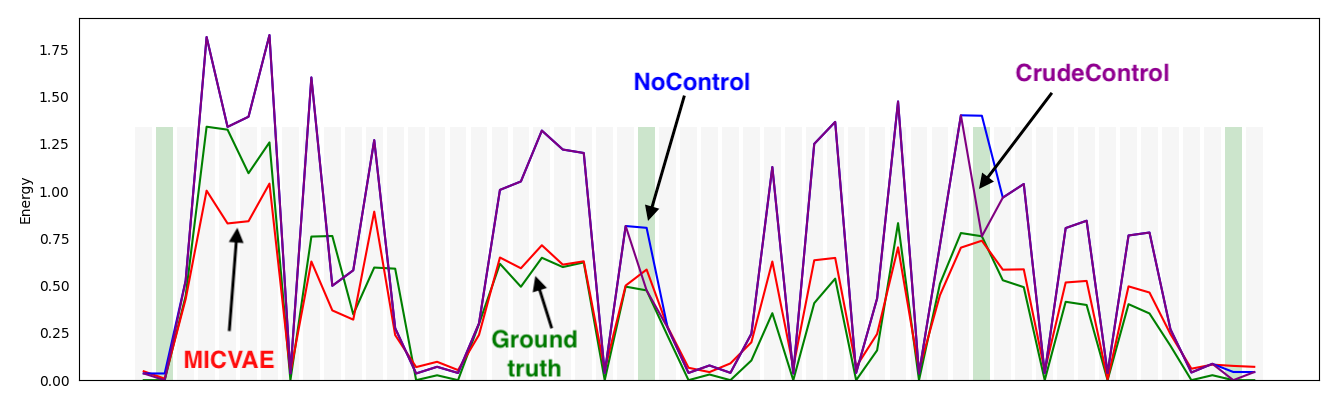
\includegraphics[width=\columnwidth]{figures/demo_a09_08q_004_energy.png}}
    \vskip -0.1in
    \caption{Our model produces plausible prosody, whereas Crude Control produces inconsistent prosody. The control points are shown with green vertical bars.} % \com{Show visually the missing PAFs.}
    \label{fig:demo}
    \vskip -5pt
\end{figure}


% We use this automated evaluation to 1) ensure that the experiments are reproducible and 2) enable larger scale experiments which would be costly to run using with humans.

We evaluate MICVAE's efficiency and robustness using a purpose-built prosody control dataset: a proprietary Latin American Spanish corpus featuring 32 speakers (17 female, 15 male) and comprising approximately 38 hours of expressive speech across ~26,000 utterances. We reserve 800 utterances for validation and 182 for testing, covering a variety of emotional and speaking styles. Data preparation involves one-hot encoding of phonetic, punctuation, and boundary tokens. Pre-emphasis is applied to waveforms, and mel-spectrograms are extracted using 128 bins, a 50ms frame length, and a 10ms frame shift. \(f_0\) is extracted using RAPT~\parencite{RAPT:1995}, and energy is calculated as the frame-wise root-mean-square of the waveform. Durations are obtained via a Kaldi forced aligner~\parencite{PoveyASRU2011}, and all features are mean-variance normalized per speaker.

Speech is synthesized using a TTS system conditioned on MICVAE's PAFs. The system includes a Latin American Spanish front-end for text normalization and grapheme-to-phoneme conversion. The acoustic model relies on Ctrl-P~\parencite{PaperCup-Ctrl-P:2021}, an attention-based Tacotron-2 variant, while the neural vocoder is WaveRNN~\parencite{waveRNN:2018}. 

Human-in-the-loop (HitL) control is simulated by selecting a subset of PAFs, referred to as control points, from one actor's rendition of a given test sentence. These control points condition our Acoustic Feature Predictor (AFP) model, with the remaining PAFs being generated by the model. We use Root Mean Square Error (RMSE) to quantify the quality of control between model-generated and ground-truth PAFs.

% The model is conditioned on control points from one actor (control speaker) but uses the speaker label from another actor (target speaker). This ensures that the control is attributable to the control points rather than the speaker label~\parencite{Sini2020IntroducingPS}.

% Our experiments aim to adapt to different prosody values during test time while controlling for possible confounds from speaker identity. To address this confound, we randomize speakers, which also happens to correspond to speaker adaptation. By performing per-speaker PAF normalization, the effect of speaker identity is primarily reflected in the relationship between prosody and text, rather than the distribution of prosody itself.

% It is important to note that, in the context of speaker adaptation, we do not explicitly focus on speaker similarity since we are dealing with vanilla TTS (with control). This implies that the test speaker must be included in the training dataset. Consequently, we do not conduct speaker similarity tests, which would be a necessary aspect of speaker adaptation research.

\subsubsection{Baselines}

\textbf{\textsc{Masked CVAE}.} Masked CVAE is a baseline system that uses the standard approach of masking for missing data imputation and inpainting~\parencite{Elharrouss2019ImageIA}. Masked CVAE has a similar architecture to MICVAE, the primary difference lies in the encoder design. Masked CVAE employs a multi-layer Recurrent Neural Network (RNN) as its encoder. Input PAFs are augmented with an additional binary feature for each of the three streams (\fzero, energy, duration) to indicate whether a given PAF is provided (1) or missing (0). Unlike MICVAE, which is inherently robust to varying levels of input missingness, Masked CVAE must be trained with sparsity in order to learn what the values 0,1 in the mask denote. During training, a fixed missingness percentage \( P \) is set, and \( P \% \) of the PAFs are randomly masked out for each training sentence.

% However, masked CVAE is not invariant to the number of control points like MICVAE is, so it generalises poorly to patterns of missingness unseen during training.

\textbf{\textsc{No Control}.} The default prosody model: predicts PAFs from phones, speaker identity, and style code. Uses the same decoder architecture as the MICVAE.

\textbf{\textsc{Crude Control}.} A na\"ive system that forcefully modifies predicted values individually, this straw-man represents a controllable model that is entirely inconsistent. Its default prosody is generated with \textsc{NoControl}, and then modified manually with the control points\footnote{Samples demonstrating TTS for these systems can be found here, \href{https://anonymous-submission-563098.github.io/sparse-control/}{anonymous-submission-563098.github.io/sparse-control}}.

\subsubsection{Evaluation Results}

\begin{figure}[t]
    \centerline{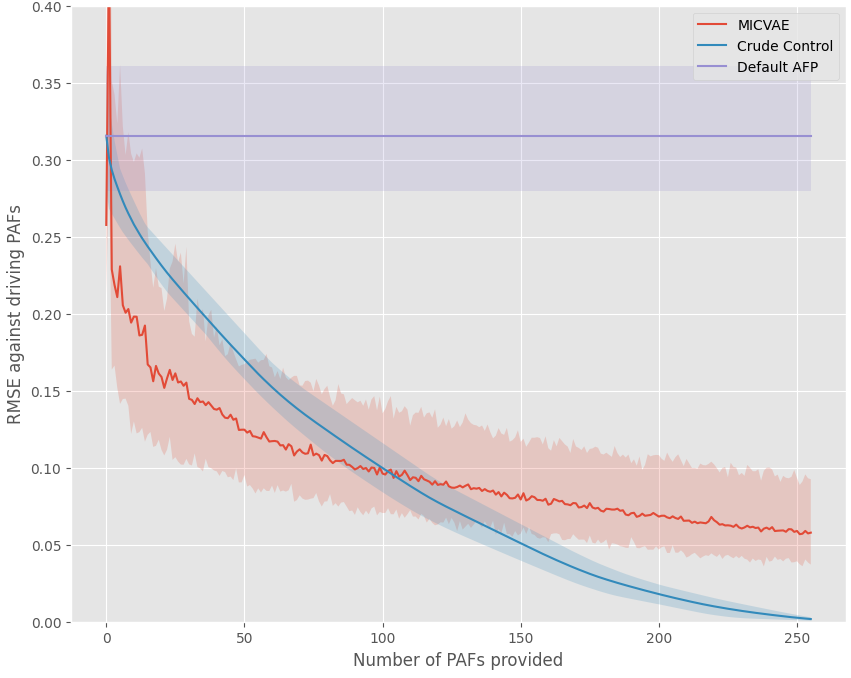
\includegraphics[width=\columnwidth]{figures/efficiency.pdf}}
    \vskip -0.15in
    \caption{Our model controls prosody efficiently. Its generated PAFs are closer to the ground-truth rendition than  is the manually modified output of the AFP, called \sc{CrudeControl}.}
    \label{fig:iterative}
    \vskip -0.2in
\end{figure}

\begin{figure}[t]
    \begin{center}
        \centerline{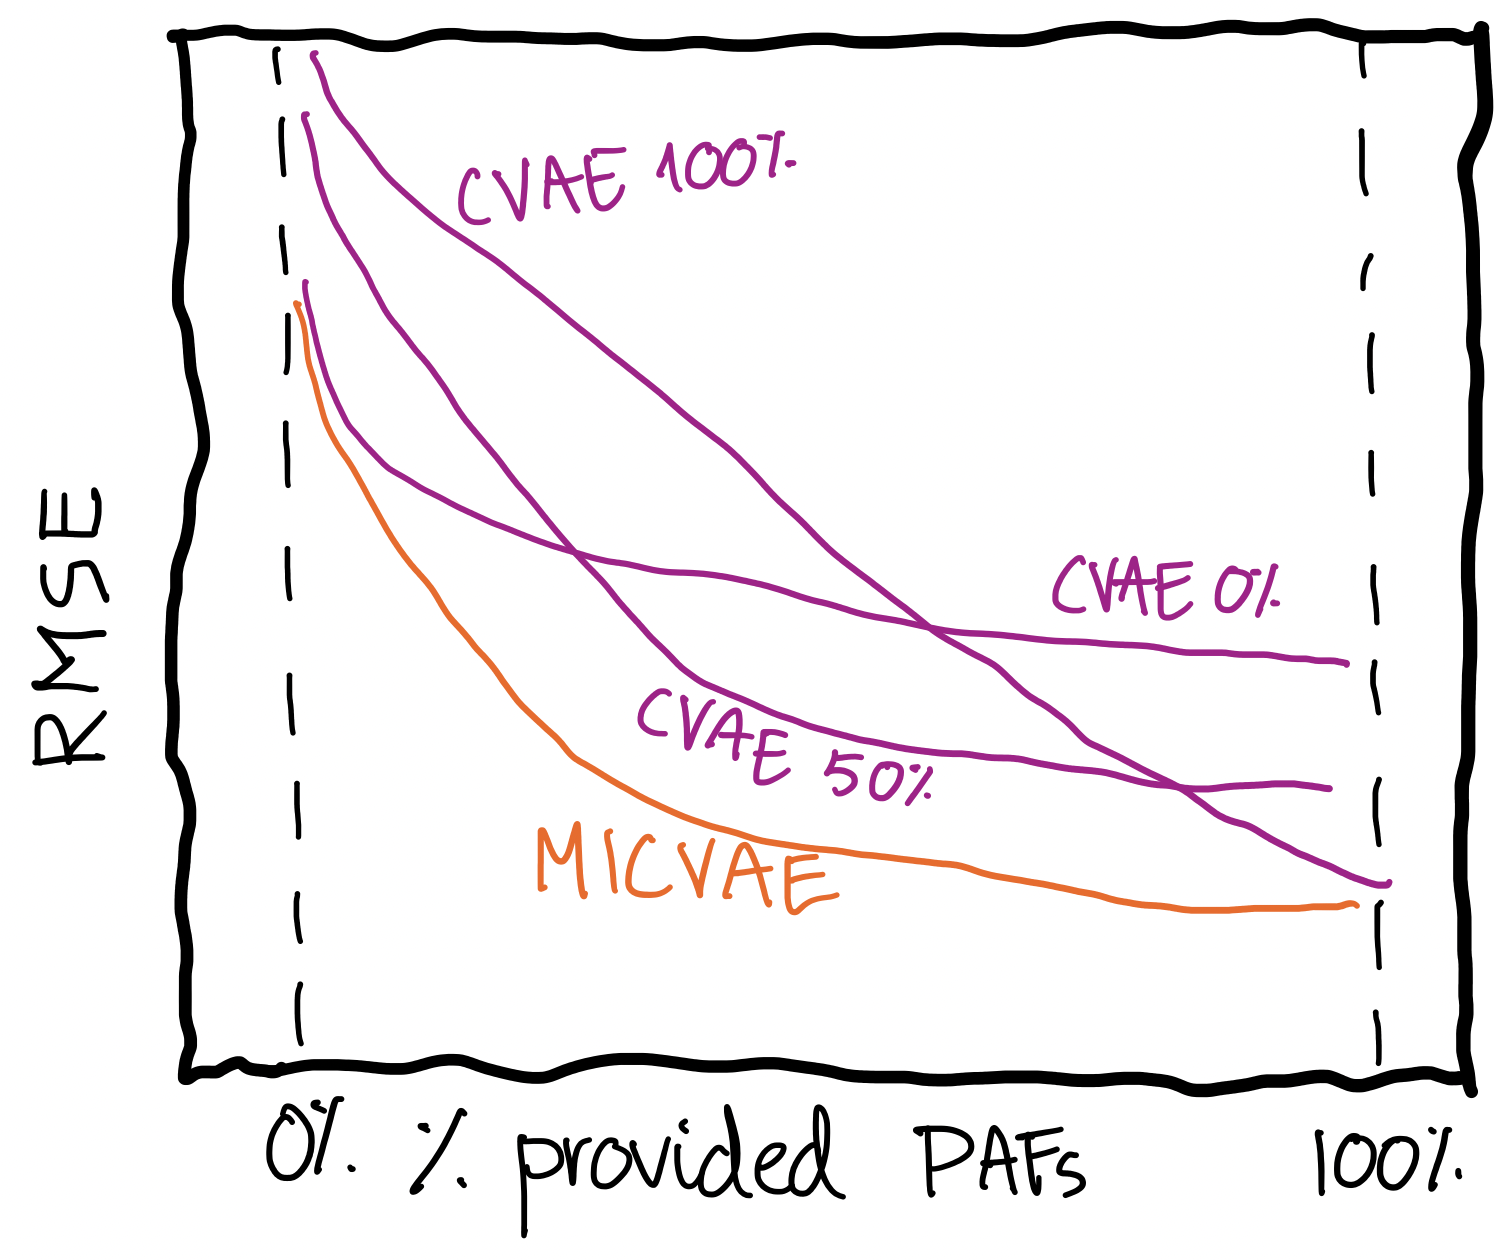
\includegraphics[width=0.9\columnwidth]{figures/robustness.pdf}}
        \vskip -0.15in
        \caption{Our model is robust to changes in the missingness pattern, whereas Masked CVAE only performs well when tested on the same missingness pattern as the one on which it was trained.}\label{fig:robustness}
    \end{center}
    \vskip -0.3in
\end{figure}

\begin{figure}
    \begin{center}
    \centerline{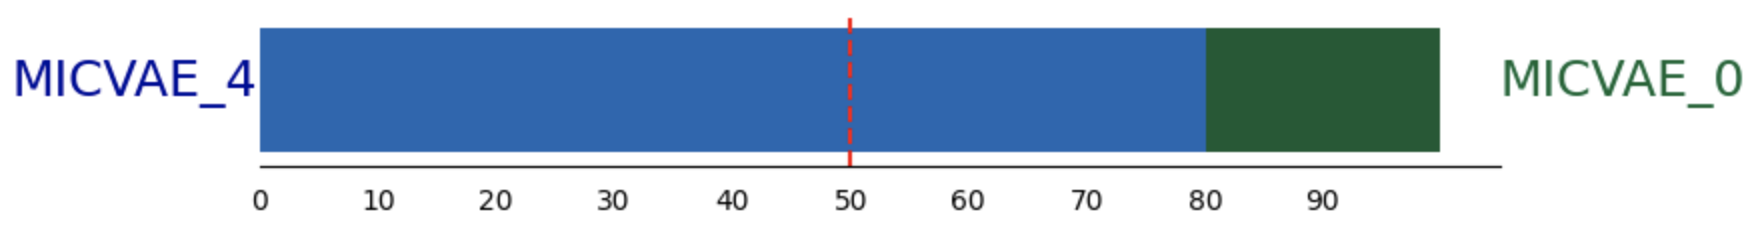
\includegraphics[width=\columnwidth]{figures/faithfulness.png}}
    \vskip -0.15in
    \caption{4 control points are enough to bring our model's output significantly closer to the reference utterance. These are ratings in an A/B/R test where the question is ``Which of these is closer to the reference ground-truth control audio?''.}
    \label{fig:faithfulness}
    \end{center}
    \vskip -0.3in
\end{figure}

\textbf{\textsc{Efficiency} (Objective Evaluation).} We assess efficiency by how many control points are required for the model to produce outputs that align with the user's intention. Alignment is measured by the Root Mean Squared Error (RMSE) between the generated and ground-truth PAFs. We feed the model with additional control points from our test set incrementally. In this ``iterative refinement'' process the PAF with the highest RMSE in the previous generation is provided in the next step. A lower RMSE achieved with fewer input PAFs directly translates to efficiency; it implies less user input is required to generate satisfactory prosodic features.

Figure~\ref{fig:iterative} reveals that MICVAE significantly outperforms the \textsc{CrudeControl} method, achieving lower RMSEs across a realistic range of missingness (between 4 and 70 PAFs). Our model (MICVAE) produces prosody closer to the ground-truth than the prosody resulting from manually setting the output PAFs to default values, meaning MICVAE uses the learned structure of prosody data to fill in the gaps between the control points. The fact that Crude Control performs better than MICVAE is to be expected when the missingness rate approaches 0, because we are manually switching all PAFs to the values extracted from the ground-truth utterance.

\textbf{\textsc{Efficiency} (Subjective Evaluation).} We also conduct an A/B/R listening test involving 20 native Latin American Spanish speakers. Participants choose which of two audio outputs (one with 4 input PAFs and one with 0) sounds closer to a reference ground-truth audio. We chose 4 and 0 to demonstrate the impact that just 4 control points can have on the prosody.

Figure~\ref{fig:faithfulness} reveals that MICVAE with 4 input PAFs is significantly perceived as closer to the reference audio compared to the version without any input PAFs. This not only confirms the model's faithfulness to user intentions but also underscores its efficiency, as it achieves these results with a minimum number of input PAFs.

\textbf{\textsc{Robustness} (Objective Evaluation).} A robust model should adapt to different missingness patterns, thereby providing users the flexibility to choose which PAFs to specify. This robustness is essential for accommodating the diversity of user input methods and intents. We examine MICVAE's robustness against varying patterns of missingness by comparing it to Masked CVAE. The evaluation involves running simulated control tests with random selections of control points at different numbers (0, 6, 12, 36, 72, 256).

As illustrated in Figure~\ref{fig:robustness}, MICVAE outperforms all versions of Masked CVAE, even with the same model capacity. The results indicate that Masked CVAEs fail to adapt to varying missingness patterns effectively, emphasizing the robustness of MICVAE. Note that our evaluation results generalise to other generative models than CVAE.\@ We compare different conditioning mechanisms (multiple-instance vs masking) rather than different generator architectures.

\subsection{Limitations}

We acknowledge that our work does not investigate all plausible strategies for selecting control points. We explored two strategies: randomly selecting a certain number of PAFs or using iterative refinement (sequentially providing all the PAFs in descending order of reconstruction error). However, other strategies exist, including: 1) Providing PAFs for an entire word. 2) Providing a few PAFs at the beginning and the end of a sentence. 3) Providing only F0 values. A detailed user study would evaluate the utility of our control framework in a range of practical settings.

Nevertheless, we believe that our quantitative evaluation already demonstrates the effectiveness of our model as a proof of concept. Our work presents a novel problem (efficiency and robustness) and approach (partial inputs) in order to initiate discussion and collaboration within the community. Future research can expand our work by conducting user studies of how humans choose to manipulate PAFs in practice.

\subsection{Conclusion}

In this study, we address the challenges of controlling generative models by introducing a new partial-input control framework. We establish three key attributes for a successful generative model: efficiency, robustness, and faithfulness. Our model, derived from the Masked CVAE, empirically exhibits these traits. To enable reproducible testing, we use simulated human-in-the-loop (HitL) control with natural prosodic features extracted from a dataset of repeated utterances. Our work serves as a foundation for future studies on human-in-the-loop control in generative models.

% \crit{A human could mimic the desired prosody within an audio sample. The reviewer's suggestion is insightful, and this technique can already be implemented within our sparse control framework. By speaking the sentence, extracting the PAFs, normalizing them and providing them as control points to MICVAE, we can already condition on audio samples. }

\section{Discussion}

%%%%%%%%%%%%%%%%%%%%%%%%%%%%%%%%%%%%%%%%%%%%%%%%%%%%%%%%%%%%%%%%%%%%%%%%%%%%%%%%
%% References:
%%
% If you include some work not referenced in the main text (e.g. using \nocite{}), consider changing "References" to "Bibliography".
%

% \renewcommand to change default "Bibliography" to "References"
% \renewcommand{\bibname}{References}
\cleardoublepage
\phantomsection
\addcontentsline{toc}{chapter}{References}
% \bibliographystyle{plainnat}
\printbibliography

%%%%%%%%%%%%%%%%%%%%%%%%%%%%%%%%%%%%%%%%%%%%%%%%%%%%%%%%%%%%%%%%%%%%%%%%%%%%%%%%
%% Appendix:
%%

%\appendix

%\chapter{Extra Information}

\end{document}
